\documentclass[11pt]{article}
\usepackage[letterpaper,margin=1in]{geometry}
\usepackage[T1]{fontenc}
\usepackage{lmodern}
\usepackage{amsmath,amssymb,amsthm}
\usepackage{booktabs,tikz}
\usepackage[bookmarksnumbered,hidelinks]{hyperref}
\hypersetup{pdftitle={Exact equilibrium in Bayesian simple security games, affine matching markets, and parallel-road traffic},
  pdfauthor={Research project coordinated by Vincent Lin}}
\urlstyle{same}
\raggedbottom
\newtheorem{theorem}{Theorem}[section]
\newtheorem{lemma}[theorem]{Lemma}
\newcommand{\Market}{\mathsf{M1}}
\newcommand{\Traffic}{\mathsf{Traffic}}
\newcommand{\BNE}{\mathsf{BNE}}
\newcommand{\dd}{\mathrel{\leq_{\mathrm m}}}
\DeclareMathOperator{\caparc}{cap}
\title{Exact equilibrium in Bayesian simple security games,\\
affine matching markets, and parallel-road traffic}
\author{Research project coordinated by Vincent Lin}
\date{November 27, 2026}

\begin{document}
\maketitle
\begin{abstract}
We give polynomial-time many-one reductions between three exact search
problems. The outputs are a Bayes--Nash strategy profile in a simultaneous
Bayesian simple security game, prices and trades in a divisible matching
market with linearly transferable utility, and a multiclass Wardrop flow
on parallel roads. The traffic model permits arbitrarily many classes and
roads, with a separate strictly increasing affine cost for every class on
every road. The two traffic reductions are direct. One represents a good's
price by the load on a road. The other uses a capacitated flow network to
represent road load by a market price. An earlier reduction from security
games to matching used adaptive market queries. We encode these queries
in a single market and recover a full game profile from every market
equilibrium. The reduction from matching to security games uses one
defender resource.
\end{abstract}

\section{Introduction}\label{sec:intro}
A traveler chooses a road of minimum cost at the prevailing loads. A buyer
chooses a good of maximum utility at the prevailing prices. Matching the
two choice rules requires a second step. A road's load is the sum of the
flows choosing it. A market price must clear a fixed capacity. We give a
construction for each direction and connect both to equilibrium in
Conitzer's simultaneous security game~\cite{conitzer}.

\begin{theorem}[Exact equilibrium search]\label{thm:traffic}
The following three search problems are equivalent under polynomial-time
many-one reductions.
\begin{enumerate}
\item Find a full Bayes--Nash profile in a Bayesian simple security game
with an integral defender budget. Coverage weakly improves the defender's
payoff and weakly reduces the attacker's payoff on the attacked target.
\item Find clearing prices, utilities, and trades in a divisible two-sided
matching market with strictly decreasing affine offers and zero outside
options.
\item Find an equilibrium matrix of class flows on two vertices joined by parallel
roads. Each class can use every road and has its own nonnegative intercept
and positive slope on each road. The numbers of classes and roads are
part of the input.
\end{enumerate}
In a reduction to security games, one defender resource and unit defender
gains suffice.
\end{theorem}

Write \(A\dd B\) if a polynomial-time transformation builds one instance
of \(B\) and a polynomial-time decoder recovers an answer to \(A\) from
\emph{every} admissible answer to that instance. All numerical data are
rationals in binary. For each search problem fix a polynomial witness-length
bound large enough to admit a basic feasible solution on each feasible
support and, for a game, a sparse realization of the defender marginals.
An adaptive oracle algorithm has a polynomial clock in the original input
length on every valid transcript, including the cost of reading answers.

\paragraph{Two direct reductions.}
Sections~\ref{sec:forward} and~\ref{sec:device} prove
\(\Market\dd\Traffic\) and \(\Traffic\dd\Market\), respectively, where
\(\Market\) denotes matching and \(\Traffic\) denotes traffic. In the
first construction, auxiliary travelers fill each good's unused capacity.
In the second, the marginal cost of a network constructed by Disser and
Skutella~\cite[Section~3.1]{ds} sets the price of an entry good. Only the
support of the resulting approximate flow is needed to recover an exact
traffic equilibrium. Meunier and Pradeau~\cite[Theorem~1]{mp} give a
polynomial algorithm for affine multiclass traffic when the numbers of
vertices and classes are fixed. Our transformations allow the number of
classes to grow with the input.

\paragraph{Why one market query suffices.}
We use \(\Market\) for Galichon and Jacquet's divisible matching model with
singles~\cite{gj}, following the notation of Lin's earlier manuscript~\cite{book}.
That manuscript embeds matching into a one-resource game and reduces general
security games back to matching by adaptive queries. Section~\ref{sec:bridge}
gives the two constructions. Appendix~\ref{sec:compile} proves that a
single market can encode a valid transcript of any such deterministic
polynomial-time oracle algorithm. Composing these reductions through
matching gives the equivalence with security-game search, denoted \(\BNE\).

\section{Models and exact recovery}\label{sec:models}

\subsection{The simultaneous security game}
There are \(n\ge1\) targets, \(m\ge1\) attacker types of prior
\(p_i\ge0\), \(\sum_i p_i=1\), and an integral defender budget \(0\le r\le n\).
We write \([n]=\{1,\ldots,n\}\).
A pure defense is an \(r\)-subset. Its mixed strategy has target marginals
in the hypersimplex
\[
 H_r=\{x\in[0,1]^n:\ \textstyle\sum_jx_j=r\}.
\]
Write \(\sigma_{ij}\) for the conditional probability with which type \(i\)
attacks \(j\). At a marginal equilibrium, each \(\sigma_i\) is supported on
maximizers of \(U_{ij}(x)=a_{ij}-b_{ij}x_j\), \(b_{ij}\ge0\), and the
defender maximizes \(\pi(\sigma)\cdot x\) on \(H_r\), where
\(\pi_j(\sigma)=d_j\sum_i p_i\sigma_{ij}\), \(d_j\ge0\). We require a
conditional best response even at a listed zero-prior type. A \emph{full
profile} specifies the defender's distribution on pure defenses and the
attacker's conditional distribution for each type. Here \(a_{ij}\) is the
type's uncovered payoff, \(b_{ij}\) its payoff loss from coverage, and
\(d_j\) the defender's gain from covering the attacked target.
Under the convention that an ex ante equilibrium leaves zero-prior rows
arbitrary, replace each such row by a maximizing pure attack. This takes
polynomial time and preserves all positive-prior choices and defender payoffs.

For the positive-prior rows let \(f_{ij}=p_i\sigma_{ij}\) denote joint
attack mass, so the score of target \(j\) is \(d_j\sum_i f_{ij}\).
A coverage \(x\) is optimal against these scores precisely when a cutoff
\(\lambda\) makes \(x_j>0\) imply \(\pi_j\ge\lambda\) and \(x_j<1\)
imply \(\pi_j\le\lambda\). Moving coverage from a lower to a higher
score proves necessity, and allocating to the largest scores proves
sufficiency. Every point of \(H_r\) is realized by a lottery on at most
\(n\) pure defenses with rational, polynomial-size support when the
marginals are rational. For example, partition \([0,r)\) consecutively
into intervals of lengths \(x_j\). A uniform \(s\in[0,1)\) selects the
half-open intervals hit by \(s,s+1,\ldots,s+r-1\). Each interval has
length at most one, so each selected set has size \(r\) and each marginal is \(x_j\).
Only fractional parts of the interval endpoints change the selected set.
The consecutive subinterval lengths in \([0,1)\) give the lottery weights.
For \(r=0\) take the empty defense.
\subsection{Parallel roads}
There are two vertices joined by parallel directed roads. Class \(i\) has
mass \(h_i>0\) of nonatomic travelers. If \(f_{ij}\ge0\) travel on road \(j\)
and \(X_j=\sum_i f_{ij}\), its cost to class \(i\) is
\(\ell_{ij}(X_j)=A_{ij}+B_{ij}X_j\), where \(A_{ij}\ge0\) and \(B_{ij}>0\).
A Wardrop equilibrium is a matrix of class flows with row sums \(h_i\)
such that \(f_{ij}>0\) implies
\(\ell_{ij}(X_j)\le\ell_{ik}(X_k)\) for every \(k\). The total mass is
\(T=\sum_i h_i\). Intermediate instances can have restricted nonempty menus,
constant costs, and signed intercepts. Existence follows from the continuous
variational inequality on the compact product of the class simplices
\cite{mp}.

For the strictly increasing costs of Theorem~\ref{thm:traffic}, the
aggregate road loads \(X\) are unique. Suppose equilibria \(f,g\) give
different loads \(X,Y\) and put \(S=\{j:X_j>Y_j\}\). Since road loads
have fixed total, \(S\) gains flow. Some class \(i\) sends more to \(S\)
under \(f\) and hence less to its complement. Choose \(j\in S\) used
by \(i\) under \(f\), and \(k\notin S\) used by \(i\) under \(g\).
Optimality at both profiles gives
\[
 \ell_{ij}(Y_j)<\ell_{ij}(X_j)\le\ell_{ik}(X_k)
       \le\ell_{ik}(Y_k)\le\ell_{ij}(Y_j),
\]
a contradiction. This parallel-road case fits the network uniqueness
results of Milchtaich~\cite{milchtaich}. The \emph{class flows} can vary.
For example, two unit classes with cost \(X_j\) on each of two roads
have loads \((1,1)\) under either assignment of one class per road.
Given \(X\), a transportation LP recovers class flows with the prescribed
row and column sums and permits only minimum-cost class--road pairs.

\subsection{Affine matching and exact support recovery}
Buyer \(i\) has mass \(m_i>0\), good \(j\) has capacity \(c_j>0\), and
a listed pair \(ij\) has utility \(a_{ij}-b_{ij}P_j\) with \(b_{ij}>0\).
The outside utility and reserve prices are zero. An equilibrium consists of
prices \(P_j\ge0\), values \(u_i\ge0\), and trades \(g_{ij}\ge0\), satisfying
\begin{align}
 u_i&\ge a_{ij}-b_{ij}P_j
       &&\text{with equality if }g_{ij}>0,\nonumber\\
 \sum_jg_{ij}&\le m_i &&\text{with equality if }u_i>0,\label{eq:m1}\\
 \sum_i g_{ij}&\le c_j &&\text{with equality if }P_j>0.\nonumber
\end{align}
Equivalently, the no-blocking inequality is
\(\lambda_{ij}u_i+(1-\lambda_{ij})P_j\ge\Phi_{ij}/2\) with
\(\lambda_{ij}=1/(1+b_{ij})\) and \(\Phi_{ij}=2a_{ij}/(1+b_{ij})\),
as in~\cite{gj,book}. An unlisted option may be given a negative intercept.
Isolated buyers and goods have value or price zero and can be reinstated
after solving. We may assume at least one listed pair.

\begin{lemma}[Recovery by linear programming]\label{lem:repair}
For a traffic or matching input, one can compute a positive integer \(Q\) of polynomial bit
length with the following guarantees.
\begin{enumerate}
\item For traffic, suppose a feasible flow uses roads of excess cost strictly
less than \(1/Q\) for their classes. Its support determines an exact rational
equilibrium in polynomial time.
\item For matching, suppose prices, values and trades satisfy the payoff and
row conditions in~\eqref{eq:m1}. Allow an additive capacity excess on any
column and an additive shortfall on positive-price columns, each less than
\(1/Q\). Assume \(P_j\le P_*:=1+\max(0,\max_{ij}a_{ij}/b_{ij})\).
The trade support and the zero/nonzero labels of prices and values then
determine an exact rational equilibrium in polynomial time.
\end{enumerate}
\end{lemma}
\begin{proof}
For traffic fix the supplied support \(S\). Keep nonnegativity, the row sums,
the load identities, and zeros off \(S\). For each \(ij\in S\) impose
\(\ell_{ij}(X_j)\le\ell_{ik}(X_k)+t\) for every allowed \(k\). Minimize
\(0\le t\le1\). For matching set unrecorded trades and zero-labeled
coordinates to zero, keep all payoff inequalities and equality on the
recorded support, and keep the row bounds with equality on positive-value
rows. Minimize \(t\) subject to \(0\le t\le1\). Impose
\(\sum_i g_{ij}\le c_j+t\) for all goods and
\(\sum_i g_{ij}\ge c_j-t\) on positive-price goods. Bound prices by \(P_*\)
and values by \(1+\max(0,\max_{ij}a_{ij})\). The latter bound holds because
a buyer with positive value uses some listed pair. No label imposes a strict
inequality in either LP.

In each model there are only polynomially many \emph{individual} rows
that can occur over all labels. Clear denominators row by row, including
the right-hand side. If \(D\) is the number of variables including \(t\)
and \(H\ge1\) bounds the resulting absolute integer entries, use
\(Q=(DH)^D\). Each feasible LP is bounded. Cramer's rule bounds the
denominator of \(t\) at an optimal vertex by \(Q\). The supplied point
permits \(t<1/Q\), so the optimum is zero. Exact rational linear programming
returns a solution. If a recorded flow or positively labeled coordinate
becomes zero, the equations imposed on it still imply the defining
equilibrium conditions.
\end{proof}

\section{From matching to traffic}\label{sec:forward}


To read a price from a traffic equilibrium, give each good its own road
and add classes of auxiliary travelers. The auxiliary travelers absorb
capacity left by original buyers. On a used road, a small change in load
then represents the good's price. At the end a support LP removes the
small errors introduced by making every road cost strictly increasing.

Choose a positive dyadic \(\tau\) with \(\tau P_*<1/(2Q_{\rm M})\),
where \(Q_{\rm M}\) comes from the matching input in Lemma~\ref{lem:repair}.
Create one road per good and a common outside road \(o\). Each original
buyer becomes a class with costs
\[
 \ell_{ij}(X_j)=-a_{ij}+b_{ij}(X_j-c_j)/\tau,\qquad \ell_{io}=0 .
\]
For each \(j\), a further class of mass \(c_j\) can use road \(j\) at cost
\((X_j-c_j)/\tau\), or \(o\) at cost zero. This class fills unused capacity
while the price is zero.

At equilibrium \(X_j<c_j\) is impossible, since then the added class alone
would send \(c_j\) there. Put \(P_j=(X_j-c_j)/\tau\). If \(P_j>0\), the
added class uses only \(o\), so the original buyers supply
\(X_j=c_j+\tau P_j>0\). Some original buyer weakly prefers \(j\) to the
outside option, giving \(P_j\le P_*\). If \(P_j=0\), original traffic on
the road is at most \(c_j\). The original flows use best offers at prices
\(P\), and a buyer with strictly positive best utility uses its entire mass
on real goods. Lemma~\ref{lem:repair} recovers an exact matching equilibrium
from the support and labels, since every column error is at most \(\tau P_*\).

It remains to obtain the intermediate equilibrium from an oracle with the
strict costs and full menus of Theorem~\ref{thm:traffic}. Compute
\(Q_{\rm W}\) for this intermediate instance and write \(T'\) for its total
mass, including the added classes. Add \(\zeta X_j\) to every allowed cost,
including that on \(o\), where \(0<\zeta<1/[2(1+T')Q_{\rm W}]\) is dyadic.
For each class add the same constant to all allowed intercepts to make them
nonnegative. On each missing road give the class a positive slope and an
intercept greater than its maximum allowed cost on \([0,T']\). No traveler
can use such a road at equilibrium. Removing the common shift and then the
perturbation leaves every used road within \(\zeta T'<1/Q_{\rm W}\) of
minimum cost for its class. The traffic LP first recovers an exact
intermediate equilibrium, and only then do we form the prices \(P_j\) and
apply the matching LP. Both dyadic precisions require polynomially many
bits. This proves \(\Market\dd\Traffic\).

\section{From traffic to matching}\label{sec:device}

The reverse reduction needs a good whose price a traveler can read as a
function of the mass assigned to its road. To achieve accuracy \(\delta\),
a direct table of prices could require \(T/\delta\) entries. We instead
use a network with \(O(1+\log(1+T)+\log(1/\delta))\) arcs. Its minimum
cost as a function of flow has one slope for each price level.

\subsection{A flow network with consecutive marginal costs}

Let \(0<\delta\le1\) be dyadic and choose the least \(k\ge1\) with
\(K=2^k\delta>T+\delta\). The network \(G_0\) has a single zero-cost arc
\(s_0\to t_0\) of capacity \(\delta\). To obtain \(G_h\), add a source
\(s_h\), a sink \(t_h\), and the four arcs in Figure~\ref{fig:count}.
Each has capacity \(c=2^{h-1}\delta\). The two positive fees both equal
\(w_h=(2^h-1)/2\). Thus \(G_k\) is acyclic and has \(4k+1\) arcs.

\begin{figure}[ht]
\centering
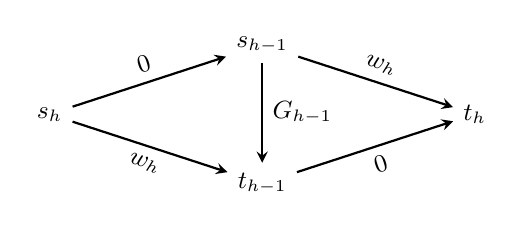
\begin{tikzpicture}[>=stealth,thick,every node/.style={font=\small}]
  \node (s) at (0,0) {$s_h$};
  \node (a) at (2.7,.88) {$s_{h-1}$};
  \node (b) at (2.7,-.88) {$t_{h-1}$};
  \node (t) at (5.4,0) {$t_h$};
  \draw[->] (s) -- node[above,sloped] {$0$} (a);
  \draw[->] (s) -- node[below,sloped] {$w_h$} (b);
  \draw[->] (a) -- node[above,sloped] {$w_h$} (t);
  \draw[->] (b) -- node[below,sloped] {$0$} (t);
  \draw[->] (a) -- node[right] {$G_{h-1}$} (b);
\end{tikzpicture}
\caption{One level of the Disser--Skutella network. The four outer arcs
have equal capacity. The vertical arrow stands for the entire preceding
network.}\label{fig:count}
\end{figure}

\begin{lemma}\label{lem:slopes}
Let \(F_h(y)\) be the minimum cost of a flow of value \(y\) in \(G_h\).
Its domain is \([0,2^h\delta]\). On successive open intervals of width
\(\delta\), its slopes are \(0,1,\ldots,2^h-1\).
\end{lemma}
\begin{proof}
The base arc gives the statement for \(h=0\). Write \(z\) for the flow
through the inner network. At outer value \(y\in[0,2c]\) the two costly
arcs together carry \(y-z\), and the two free arcs together carry \(y+z\).
Thus \(0\le z\le\min(y,2c-y)\). Every such \(z\) is feasible by placing
\((y-z)/2\) on each costly arc and \((y+z)/2\) on each free arc.
Consequently
\[
 F_h(y)=\min_{0\le z\le\min(y,2c-y)}
             \{w_h(y-z)+F_{h-1}(z)\}.
\]
The largest inner slope is \(2^{h-1}-1<w_h\), so the largest feasible \(z\)
is optimal. The first half keeps the inner slopes. The second half has the
slopes \(2w_h-(2^{h-1}-1),\ldots,2w_h\) in that order.
\end{proof}

\subsection{Representing the marginal cost by a market price}

For one road construct a set of private buyers and goods and a single
\emph{entry good} \(p\). Only \(p\) is offered to the traffic classes.
Let \(X\in[0,T]\) denote their total purchases of \(p\), and \(\pi\) its
price. Put \(s=s_k\), \(t=t_k\), \(C=T+\delta+1\), and write
\(\kappa_e\) for an arc's fee. Define
\[
 \kappa'_e=\kappa_e+\mathbf1_{\{\operatorname{head}(e)=t\}},
 \qquad M=4+\sum_e\kappa'_e,\qquad M_p=M+1.
\]
Each arc \(e\) becomes a good of capacity \(\caparc(e)\), available only
to its two endpoints. All private offers have the form
\(\text{intercept}-\text{price}\). The available offers are as follows.

\begin{center}
\small
\begin{tabular}{@{}lll@{}}
\toprule
Buyer & Mass & Goods and their intercepts\\
\midrule
Internal node \(v\) & Sum of incoming capacities &
  Incoming \(M\), outgoing \(M-\kappa_e\)\\
Source \(s\) & \(C\) & Outgoing \(M-\kappa_e\), entry \(p\) at \(M_p\)\\
Sink \(t\) & \(K\) & Incoming \(M+1\), discard good at \(M\)\\
Additional buyer & \(\delta\) & Entry \(p\) at \(M_p+1\) only\\
\bottomrule
\end{tabular}
\end{center}
The entry good has capacity \(C\), and the private discard good has
capacity \(K+1\). The latter always has price zero.

\begin{lemma}[Price as a function of load]\label{lem:price}
In every equilibrium of a market containing this construction, provided
the external buyers can purchase only \(p\) among these goods and contribute
at most \(T\), the entry price satisfies
\[
                         X\ \le\ \delta(\pi-2)\ \le\ X+\delta .
\]
\end{lemma}
\begin{proof}
If \(\pi>M_p\), the source buys none of \(p\), and all other buyers together
can supply at most \(T+\delta<C\), contradicting clearance at a positive
price. Hence the additional buyer strictly prefers to trade and buys
\(\delta\). Set \(r=X+\delta\). In particular
\(0<r<\min(C,K)\), including at the endpoints \(X=0,T\).

Remove all buyers at \(p\) except the source, keeping the other private node
buyers, and reduce its capacity to \(u=C-r\). The private allocations and
prices remain an equilibrium of this residual market. Since every remaining
offer has unit slope, these are primal and dual optima for the assignment
LP maximizing the sum of intercepts times trades, subject to buyer mass and
good capacity upper bounds. Indeed, the dual variable of a buyer is its
value, the dual variable of a good is its price, and~\eqref{eq:m1} is
complementary slackness. Write \(V(u)\) for the optimal value. We compute
it for every \(r\) in the open interval above.

\emph{Private arc goods fill.}
Take any optimal primal and dual pair for the residual market. A slack arc
good has price zero. At its head, the purchase of that arc is smaller than
its capacity. More generally, consider any zero-price incoming arc with this
property. If its head is internal, its buyer attains its largest possible
utility \(M>0\), so must spend its full mass. Its incoming purchases alone
cannot do so. It buys some outgoing arc of zero fee and zero price. At the
next head that arc again has head purchase below capacity. At the sink, a
zero-price incoming arc gives utility \(M+1\), strictly above the discard
offer. The sink must buy its full mass \(K\) on incoming arcs, whose total
capacity is exactly \(K\). This forces every head purchase there to equal
capacity. Acyclicity now contradicts the existence of the first slack arc.

\emph{Welfare of the residual market.}
Write \(f_e\) for the tail's purchase of arc \(e\). Its head buys
\(\caparc(e)-f_e\). Let \(y\) be the source's entry purchase and \(z\) the
sink's discard purchase. After subtracting a constant independent of \(u\),
the objective is
\[
                M_p y-\sum_e\kappa'_e f_e+Mz .
\]
The remaining restrictions are \(0\le f_e\le\caparc(e)\),
\(0\le y\le u\), \(y+\operatorname{out}(s)\le C\),
\(\operatorname{out}(v)\le\operatorname{in}(v)\) internally, and
\(0\le z\le\operatorname{in}(t)\). These conditions are also sufficient
for an allocation with full arc goods. In an optimum
\(z=\operatorname{in}(t)\).

First \(y=u\). Otherwise use spare source mass to increase \(y\), or, if
the source is full, follow a positive-flow path from it to a vertex with
surplus inflow or to the sink. Reduce a small amount of flow along this
path and assign the freed mass to \(p\). If the path ends at the sink,
reduce \(z\) by the same amount. The sacrifice per unit is at most \(M\)
and the entry purchase gains \(M_p>M\). This proves the assertion, leaving
\(\operatorname{out}(s)\le r<K\).

There can be no internal surplus inflow. From a surplus vertex the residual
network reaches \(s\) by tracing a positive-flow path backwards. If it could
not reach \(t\), its reachable set would contain \(s\) and exclude \(t\).
Every arc leaving the set would be saturated and every arc entering it
empty. Its cut capacity would equal its net outflow, at most
\(\operatorname{out}(s)\le r<K\), since internal nodes have no net outflow.
This contradicts the feasible flow of value \(K\) from Lemma~\ref{lem:slopes}.
Push a small amount on a simple residual path from the surplus vertex to
\(t\), increasing \(z\). The gain per unit is at least
\(M-\sum_e\kappa'_e>0\). The same cut argument starting at \(s\) shows
that \(\operatorname{out}(s)<r\) would allow a profitable push using spare
source mass. Thus the optimum conserves at every internal node and sends
exactly \(r\) to \(t\). Conversely, every feasible \(s\)-\(t\) flow of
value \(r\) yields a residual allocation with \(y=u\) and \(z=r\).
Its minimum fee sum is \(F_k(r)\), and the extra unit in \(\kappa'_e\)
is paid once per unit entering \(t\). We have proved
\begin{equation}\label{eq:value}
 V(C-r)=\mathrm{constant}+M_p(C-r)+(M-1)r-F_k(r).
\end{equation}

\emph{Price at every dual optimum.}
The dual with entry multiplier \(\pi\) stays feasible if the capacity
changes to \(u'\). Hence \(V(u')\le V(u)+\pi(u'-u)\). Substituting
\eqref{eq:value} and varying \(r\) on both sides gives
\(\pi=M_p-M+1+\mu=2+\mu\) for some \(\mu\in\partial F_k(r)\), the interval
of supporting slopes. In particular when \(r/\delta\in(l,l+1)\) we have
\(\mu=l\), and at an interior breakpoint \(r/\delta=l\) we have
\(\mu\in[l-1,l]\). Both cases give \(r-\delta\le\delta\mu\le r\).
Since \(r=X+\delta\), this is the desired inequality.
\end{proof}

\subsection{Recovering exact class flows}

For a traffic instance, compute its \(Q_{\rm W}\) and put \(B_*=\max_{ij}B_{ij}\).
Choose a positive dyadic \(\delta\le1\) with \(2B_*\delta<1/Q_{\rm W}\).
Make one independent copy of the preceding market construction per road.
For each class add a buyer of mass \(h_i\) whose offers on the entry goods
are
\[
 R_i-A_{ij}-B_{ij}\delta(\pi_j-2),\qquad
 R_i=1+\max_j\{|A_{ij}|+B_{ij}(T+1)\}.
\]
These offers have strictly positive price slopes \(B_{ij}\delta\) in
the matching convention \(a-bP\). The a priori bound \(T\) suffices for
Lemma~\ref{lem:price} even before establishing that the class buyers spend
all their mass. That lemma now implies that all displayed offers are
strictly positive. Every class spends its entire mass.

Read the class purchases as \(f_{ij}\). The cost used by the market lies
between the true cost \(A_{ij}+B_{ij}X_j\) and that cost plus \(B_*\delta\).
For a used road \(j\) and any competing road \(k\), the true cost on \(j\)
is at most the displayed cost on \(j\), hence at most the displayed cost
on \(k\). The excess relative to the true cost on \(k\) is therefore at
most \(B_*\delta<1/Q_{\rm W}\). The traffic LP recovers exact class flows.
The depth \(k\) is polynomial in the input length, as are the bit lengths of
all fees, capacities and offers. This proves \(\Traffic\dd\Market\) and
completes the two direct traffic reductions in Theorem~\ref{thm:traffic}.

\paragraph{An example of support recovery.}
Let classes of masses \(1/4\) and \(3/4\) have costs
\((X_L,2+X_R)\) and \((2X_L,1/4+X_R)\) on two roads. The first class uses
only \(L\). If the second class sent everyone to \(L\), it could lower
its cost from \(2\) to \(1/4\) on \(R\). If it sent everyone to \(R\),
it could lower its cost from \(1\) to \(1/2\) on \(L\).
It therefore uses both roads. Its indifference equation and
\(X_L+X_R=1\) force \(X_L=5/12\), \(X_R=7/12\). The second class sends
\(1/6\) to \(L\) and \(7/12\) to \(R\). This calculation illustrates what the
decoder takes from the market. Knowing which roads carry each class is
enough to reconstruct the exact loads without rounding their numerical values.

\section{Between security games and matching markets}\label{sec:bridge}

In a market a positive price forces a good to fill. In a game with one
resource and unit defender gains, positive coverage forces a target to
receive maximum attack mass. Calibrating that maximum lets coverage
encode prices.

\begin{theorem}[Matching and security games]\label{thm:bridge}
\(\Market\dd\BNE\) with one defender resource and unit defender gains.
Conversely \(\BNE\dd\Market\) for every permitted budget, including games
with zero payoff slopes or zero defender gains.
\end{theorem}

\subsection{How a one-resource game encodes a market}
We give the embedding of \cite[Theorem~3.16]{book}, using a common price
scale that permits every original slope. Remove isolated vertices and
restore their zero utilities or prices at the end. If no pairs remain,
the zero allocation and potentials solve the input. Otherwise let
\begin{align*}
 D&=1+\max\bigl(\textstyle\sum_i m_i,\max_j c_j\bigr), &W&=4D,\\
 A&=1+\max(0,\max_{ij}a_{ij}), &\gamma&=\min(1,\min_{ij}b_{ij}),\\
 S&=\bigl(1+(|I|+|J|)A\bigr)/\gamma .
\end{align*}
Here \(I,J\) index the buyers and goods. Make one real target per good,
a private target \(g_i\) per buyer, an outside target \(o\), and a control
target \(h\). Normalize the following weights by their sum to get the
attacker priors. Each unlisted payoff at target \(k\) is \(-2-x_k\).
\begin{itemize}
\item Source type \(i\) has weight \(W+m_i\), real offers
\(a_{ij}/S-b_{ij}x_j\), private offer \(A/S-x_{g_i}\), and outside offer
\(-x_o\).
\item Dedicated type \(j\), of weight \(W-c_j\), receives \(2-x_j\) on
its real target. The control type, of weight \(W\), receives \(2-x_h\) at \(h\).
\end{itemize}
Measure attacks in the original weight units. The dedicated types and the
control type always choose their designated targets, so the maximum load is
at least \(W\). Each source has an outside offer of at least \(-1\), so
it never uses an unlisted option, whose payoff is at most \(-2\).
Each source sends at least \(W\) to its private target. If that target
is covered it has maximum load and only its source can use it.
If uncovered, its offer \(A/S\) strictly beats every alternative. Thus at
most \(\sum_i m_i<W\) reaches \(o\), giving \(x_o=0\) and a nonnegative
best payoff for each source. Any covered real target needs a source buyer,
since its dedicated load is below \(W\). Its coverage is therefore at most
\(A/(\gamma S)\). Covered private targets have coverage at most \(A/S\).
The total of these coverages is strictly less than one, so \(h\) has
positive coverage. Its load is \(W\), which therefore is the maximum.
An uncovered private target would attract \(W+m_i>W\). Each private
target consequently receives exactly \(W\) and is covered.

Read \(P_j=Sx_j\), take \(u_i\) to be \(S\) times the source's best payoff,
and let \(g_{ij}\) be the source mass attacking real good \(j\). No real
target receives more than \(c_j\) source units, and every covered real
target receives exactly \(c_j\). A source with positive payoff sends its
remaining \(m_i\) units to real targets. The source comparisons now give
\eqref{eq:m1}.

Conversely, given a market equilibrium, set \(x_j=P_j/S\),
\(x_{g_i}=(A-u_i)/S\), and \(x_o=0\). A positively priced good has a
tight trade and hence \(P_j\le A/\gamma\). Every utility lies in
\([0,A)\). The remaining coverage assigned to \(h\) is positive. Each
source sends \(W\) to its private target, the real trades to the real
targets, and its unused mass to \(o\). All purchased options have best
payoff and all covered targets have maximum load. The game is finite,
so existence of a mixed Nash equilibrium and the forward decoder also
give market existence. All weights, offers, and the common price scale
have polynomial binary length.

\subsection{From a game to adaptive market queries}

For positive defender gain \(d_j\), an optimal defense has a cutoff
\(\lambda\). At interior coverage the attack load on \(j\) equals
\(\lambda/d_j\). At zero coverage it is at most this amount and at full
coverage it is at least this amount. Fixing \(\lambda\) therefore gives
a market with prices in \([0,1]\). Its buyer comparisons are the
attacker comparisons. To represent an equilibrium of the game, its prices
must also sum to the defender budget \(r\).

Here is how the adaptive construction in \cite[Theorem~3.1]{book} handles
the price sum. Assume first that the priors, slopes and defender gains are
positive and \(0<r<n\). A box \([l,h]\) with capacities
\(c_j=\lambda/d_j\) requires full best-response rows, load at least
\(c_j\) at \(x_j>l_j\), and load at most \(c_j\) at \(x_j<h_j\).
Fixing \(l_j=h_j\) leaves that column load free.

For \(\lambda>0\) one ordinary market answers this box query. Give buyer
\(i\) outside value \(v_i^0=\max_k(a_{ik}-b_{ik}h_k)\) and good \(j\)
reserve \(l_j\) by using ordinary intercepts
\(a_{ij}-b_{ij}l_j-v_i^0\) and reading \(x_j=P_j+l_j\).
If \(x_j>h_j\), strict decrease makes every offer on \(j\) worse than
its buyer's outside option, contradicting clearance of that positive-price column.
A buyer with spare mass has value \(v_i^0\) in the original units.
Every maximizer \(k\) in its reserve formula is at its ceiling, since
otherwise its offer would exceed \(v_i^0\). Assign spare mass to one
such \(k\). Only ceiling columns receive the extras, as the box requires.

At \(\lambda=0\) use the all-one corner with any best responses. At
\(\lambda=1+\max_jd_j\) the all-zero corner works because each
capacity exceeds the total attack mass. Bisect, retaining one answer
whose price sum is at least \(r\) and one whose price sum is at most
\(r\). The pattern of each endpoint fixes permitted positive edges,
zero or unit prices, and equality of load to \(\lambda/d_j\) at free
prices. Include the endpoint's sum inequality and the initial cutoff bounds
\(0\le\lambda\le1+\max_j d_j\). These closed constraints define a rational
polytope in \((\lambda,x,f)\). Its projection on \(\lambda\) is an
interval with endpoints of denominator at most a uniform \(Q\) from
the original row data, by the determinant bound of Lemma~\ref{lem:repair}.
When the sampled cutoffs are closer than \(1/Q^2\) the two intervals
meet, since distinct rational endpoints would be at least \(1/Q^2\)
apart. This yields both sum inequalities at one exact cutoff.

To order and then narrow these prices, use the following demand
comparison. On \(D=\{j:x_j>y_j\}\) the decrease from \(x\) to \(y\)
strictly improves every offer, while off \(D\) no offer improves.
Any buyer using \(D\) at \(x\) consequently uses only \(D\) at \(y\).
For two clearings at the same capacities, the box inequalities give the
opposite load comparison on each \(j\in D\). Thus the total loads on
\(D\) agree, and precisely the same buyers send their full mass to \(D\)
at both endpoints. The coordinatewise minimum takes the cheaper
columns of each clearing and their flows. The buyers confined to \(D\)
prefer their \(y\)-choices to their \(x\)-choices. The other buyers can
obtain their \(y\)-value off \(D\) at \(x\). The maximum takes the
dearer columns, where each selected choice keeps its price and no
competitor becomes cheaper. Both patched flows are equilibria. This
gives an ordered bracket \(L\le H\) with \(\sum L_j\le r\le\sum H_j\).

Pin a wide coordinate \(k\) to a dyadic price in the middle third of
\([L_k,H_k]\) and solve the smaller box \([L,H]\) with this pin.
If its load on \(k\) is at least \(c_k\), compare with \(L\) on
\(D=\{j:x_j>L_j\}\). Each column there has load at least \(c_j\) in the
new solution and at most \(c_j\) at \(L\). The demand comparison forces
equality and isolates the buyers on \(D\). Use the new columns on \(D\)
and the old ones elsewhere. If the pinned load is at most \(c_k\),
compare with \(H\) on \(\{j:x_j<H_j\}\) and use the new columns on
that set. At the new prices the other buyers have a best choice off
the set, whose prices agree with \(H\). Their old best choices there
remain optimal. Both cases recover a full-box equilibrium at the given
pin. When the cutoff is zero the upper corner of the pinned box already
answers the smaller-box query. Keep the side of the bracket containing
the desired total. Its \(k\)-width falls to at most two thirds of its old value
and other widths cannot grow.

Finally fix the lower endpoint's flow, its zero and unit labels and
the payoff comparisons on its support. Minimize the absolute budget
error over the resulting price LP in \([0,1]^n\). Its rows use only
original data and its positive optimum, if any, is at least \(1/Q'\)
by a second determinant bound. Once every width is at most
\(\eta=1/(4nQ')\), the lower endpoint exhibits error at most \(n\eta\).
The optimum is zero and the repaired prices with the saved flow are a
BNE. There are \(O(n\log(1/\eta))\) narrowing calls, with pins on a
fixed dyadic grid finer than \(\eta/4\). To bound all query lengths,
first replace each returned price by a vertex on its support and box
labels, then patch. In a tree of tight comparisons every price is
an affine function of one root, with coefficients from the original
payoff data along a path of length at most \(n-1\). At a vertex the root
is either one box endpoint or pin, or is fixed by a further tight
comparison with original coefficients. Thus each round adds polynomially
many bits to the maximum previous endpoint length. The corresponding
flow vertex depends only on margins and the fixed cutoff.

Endpoint budgets have fixed coverages. Zero-prior types can be restored
with a conditional best response. For zero slopes or gains add a common
positive dyadic \(\epsilon\) to those payoff coefficients (adding it to
all slopes and gains also works). In the original game the perturbed
support and price labels have attacker comparison error at most
\(2\epsilon\) and defender score error at most \(\epsilon\), since
\(x_j\in[0,1]\) and each load is at most one. Relax the original closed
pattern by one slack in these inequalities, leaving rows and budget
exact. The same basis argument bounds positive optimum slack below by
\(1/Q_0\) for an input-computable integer \(Q_0\) of polynomial bit
length. Taking \(2\epsilon<1/Q_0\)
recovers an exact original-game solution by LP. These are the pattern
and bit bounds of \cite[Section~3.1]{book}.

Appendix~\ref{sec:compile} gives the step from an adaptive procedure to
one market. It isolates each stage's answer, represents its relevant
rational comparisons by Boolean signals in ordinary goods prices, and
uses those signals to select the next stage's coefficients. The decoder
uses the resulting transcript to recover a complete witness. The isolation and the separation bounds ensure
that every solution of this \emph{single} market decodes. This establishes
the reverse direction in Theorem~\ref{thm:bridge}. Composing the two
game reductions with Sections~\ref{sec:forward} and~\ref{sec:device}
proves Theorem~\ref{thm:traffic}.

\appendix
\section{Encoding adaptive queries in a single market}\label{sec:compile}


The proof of Theorem~\ref{thm:compile} uses three steps. First, perturb a
query so that it has a unique answer and its set of tight offers determines
an answer to the original query. Next, place the query inside a larger market
whose earlier goods select its data. Its prices need only be accurate enough
to distinguish a zero slack from a positive one. Finally, encode these
comparisons as exact bits and use them to specify the next query. The
capacity estimates below account for the purchases made by each later
reader of an earlier good.

\begin{lemma}[Isolation of a market]\label{lem:isolate}
An ordinary market reduces in one call to a market on the same graph
with unchanged capacities and slopes and a unique real equilibrium.
Its tight graph is a forest. Exactly one vertex of each tree has zero
utility or price. A rational LP recovers an original equilibrium.
\end{lemma}
\begin{proof}
Choose a positive common denominator \(Q\) for the input data. Number
the edges \(1,\ldots,|E|\). Add \(\delta\) to each buyer mass and
\(\delta^e\) to intercept \(e\), for a small dyadic \(\delta>0\).
For a nonempty buyer set \(D\) and any good set \(S\), the difference
of their old total margins is in \(Q^{-1}\mathbb Z\). The change
\(|D|\delta\) lies in \((0,1/Q)\), so their new totals differ.

Suppose two equilibria have price vectors \(p,q\), and let
\(S=\{j:p_j>q_j\}\). If \(S\) is nonempty, it fills at \(p\). Every
buyer who buys in \(S\) at \(p\) strictly prefers \(S\) to all other
options at \(q\), since its used offer improves and every outside offer
weakly worsens. At \(p\) these buyers supply all the capacity of \(S\),
so their total mass is at least that capacity. At \(q\) they spend their
full mass there, so it is at most that capacity. Equality contradicts
the perturbed margin condition. Switching \(p,q\) proves unique
prices. The best offers then fix utilities.

Consider all tight offer equations and all zero-coordinate equations at
these potentials. Their normals are independent. Otherwise a minimal
dependence includes an offer, since the zero-coordinate normals alone are
independent. After clearing rows, its integer coefficients can be taken as
signed minors. Consistency of the right-hand sides gives a polynomial in
\(\delta\) whose distinct offer powers have nonzero coefficients. A
sufficiently small positive dyadic cannot be its root. Every connected
component of tight edges has a zero coordinate, since otherwise all its
positive margins would fill internally. A component on \(v\) vertices
has at least \(v-1\) edges and at most \(v\) independent equations
including the zero coordinates. It is a tree with one zero coordinate.
Every other margin fills, so deleting leaves towards that vertex
determines the allocation uniquely.

For recovery use the old inequalities. For each positive perturbed
coordinate impose equality in its complementary inequality, and set
each zero coordinate to zero. Every feasible solution is an original
equilibrium. To see feasibility, clear all rows by \(Q\), keep
nonnegativity, relax each row by a common slack \(t\ge0\), and minimize
\(t\). A positive optimum is at least \(1/B\) by the vertex determinant
bound, whereas the perturbed solution is feasible with \(t=Q\delta\).
For explicit sizes let \(s=|E|+|I|+|J|+1\), let \(H\ge5\) bound \(Q\)
and all absolute cleared entries, and take \(B=(sH)^{s+2}\). This bounds
the minors above as well. After clearing the tight equations the coefficients
of their consistency polynomial are integers of magnitude at most \(sHB\).
Following its least nonzero power, the tail is smaller in magnitude than
its nonzero integer coefficient if \(sHB\,\delta/(1-\delta)<1\).
Choosing \(\delta<1/\max(8,2(|I|+1)Q,2QB,4sHB)\) meets all three
requirements and gives all powers polynomial binary length.
\end{proof}

\subsection{Computing with the prices of ordinary goods}

Represent a signed number by a good's price minus a known offset. A gate
will enforce a minimum or maximum of a finite list of increasing affine
functions of earlier prices. Choose the output offset so each physical
threshold \(T_l(p_l)=A_l+B_l p_l\), \(B_l>0\), is at least one on
nonnegative prices. Choose \(U\) at least one above every threshold on
the input price ranges of interest. Make the output good capacity \(K\)
and give a unit-mass guard the sole offer \(U+1-p\) there. For a minimum,
one buyer of mass \(K\) has output offer \(U-p\) and input offers
\(U-T_l(p_l)\) for all \(l\). If two pins of a minimum refer to the
same good, insert distinct unary identity copies before the gate. Each
listed buyer--good pair then has just one offer. These copies count in
the reverse capacity calculation below. For a maximum use one such buyer per input,
each seeing only that input and the output. All buyers have their usual
outside option. Choose capacities in reverse circuit order so all readers
of this output together have mass \(<K-1\), allowing for external
readers as well. For binary gates, taking \(K\) greater by two than the
total mass already allocated suffices, with at most constant-factor
growth per gate. Reserve extra capacity for stated external reader bounds.

At price zero the guard and generators strictly want the output and exceed
its capacity. At a positive price it fills. Readers and the guard supply
strictly less than \(K\), so a generator buys there. This gives \(p\le U\)
and makes the guard buy its full unit. The aggregate generator purchase
is therefore strictly between zero and \(K\).
For a generator \(g\) with input set \(D_g\), put
\(c_g=\min(U,\min_{l\in D_g}T_l(p_l))\). Its output offer is \(U-p\).
If \(p<c_g\), that offer strictly beats all alternatives, including the
outside option, so \(g\) sends all \(K\) units to the output. If \(p>c_g\), it sends zero. In particular, positive purchases imply \(p\le c_g\).
The aggregate bounds rule out \(p<\max_g c_g\) and \(p>\max_g c_g\),
respectively. Thus \(p=\max_g c_g\). One generator with all inputs gives
the clipped minimum. One generator per input gives the clipped maximum.
On the designated range no clipping occurs. A constant \(c>0\) is fixed
by a good of capacity \(K\) with one buyer of mass \(2K\) offering
\(c-p\), subject to total reader mass \(<K\). Translation handles signed
constants. Exact bits and their complements use separate goods. AND and
OR are minima and maxima, and negation exchanges the two goods.

\begin{lemma}[Adding price signals]\label{lem:sum}
Suppose two signed input prices have logical values \(v,w\) in known bounded
ranges and \(|v-w|\le D\) for a positive power of two \(D\). For any dyadic
\(\eta>0\), a circuit with \(O(1+\max(0,\log_2(D/\eta)))\) min, max, and unary
affine gates produces a signal within \(\eta\) of \(v+w\).
\end{lemma}
\begin{proof}
Set \((v_0,w_0)=(v,w)\) and \(D_i=D/2^i\). At step \(i\) compute
\[
 v_{i+1}=\max(v_i,w_i)-D_i/4,\qquad
 w_{i+1}=\min(v_i,w_i)+D_i/4.
\]
The sum stays constant. The new absolute difference is
\(\bigl||v_i-w_i|-D_i/2\bigr|\le D_i/2\), including when the two
inputs coincide. Take the least \(h\ge0\) with \(D_h\le\eta\) and output
\(2v_h\). Its error is \(|v_h-w_h|\le\eta\). Each layer shares both
computed outputs with the next. All intermediate values stay between the
input range endpoints enlarged by \(D\) on either side, since their mean
is fixed and their difference is at most \(D\). Choosing offsets and
ceilings for this range keeps each gate in its intended operating range.
All shifts are dyadic with polynomial binary length in the input bounds
and the requested precision.
\end{proof}

\subsection{A market with coefficients selected by input bits}

\begin{lemma}\label{lem:program}
Given polynomial bounds on dimensions and coefficient bit lengths, a fixed
ordinary market module can represent any isolated query of that size. Its
data are selected by exact bit goods in earlier modules. For a prescribed
dyadic \(\zeta>0\), its output prices approximate the unique query prices
within \(\zeta\) whenever the total mass of later buyers is below a
computable positive tolerance. The module, including the binary length
of this tolerance, has size polynomial in the bounds and \(\log(1/\zeta)\).
\end{lemma}
\begin{proof}
Pad the abstract query with positive-margin isolated vertices and encode
missing edges by negative offers. Use a common positive power of two
to scale offers so all possible slopes are at least one. This leaves
good prices invariant. Choose \(H\) uniformly above all possible positive
ratios \(a_e/\beta_e\) by at least two. Build a private unary chain for
each possible pair. Its logical output approximates
\(\beta_eP_j-a_e\) within \(\xi<1/4\) on \([0,H]\). A binary choice
between two affine laws uses two equal-mass generators in place of one.
Each has an extra offer on its own earlier bit good, strictly better than
all local options in the disabling state and below zero in the enabling
state. The complementary bits enable exactly one generator. Such an
offer is decreasing affine in the physical bit price, using its known
offset and the finite upper bounds on the local intercepts. The disabled
buyer's entire mass goes to the earlier good. The active generator and
guard enforce exactly the clipped unary gate law just proved.

For each source copy, offer on its final edge good its offset minus that
good's physical price. The effective source payoff then approximates
\(a_e-\beta_eP_j\). A guard or enabled generator buys only in its own
chain or on its terminal. Disabled buyers are accounted for solely as
readers of earlier bit goods.

To encode a slope \(\beta\ge1\), first program the exponent of
\(2^{\lfloor\log_2\beta\rfloor}\) by its binary digits, selecting a
multiplier \(1\) or \(2^{2^k}\) at position \(k\). To approximate the
remaining factor in \([1,2)\) from below, at step \(k=1,2,\ldots\)
use the largest of zero, one or two factors \(1+2^{-k}\) that keep
the product below or equal to the requested factor. The remaining ratio
is at most \(1+2^{-k}\), since
\((1+2^{-k})^2\ge1+2^{-(k-1)}\). Stop once
\((\max\beta)H2^{-k}<\xi/2\). Translate by dyadic digits for \(-a_e\)
with error \(<\xi/2\). Use program-independent positive offsets and gate
ceilings computed forward for both possible branches. A fixed, padded
chain thereby covers every possible query word. The bit choices follow
from rational comparisons of polynomial-length numbers.

Represent masses by enabled binary-weight copies of each source buyer,
with the same offers on its roots, and approximate each margin to
accuracy \(\xi\) on a common dyadic grid. Take \(\xi\) below half every
possible positive margin. At terminal \(j\) use binary-weight singleton
buyers offering \(H+1-P_j\) to preload the difference
\(C-\widehat c_j\) between a fixed ceiling \(C\) and the programmed
capacity. Disabled copies and singleton buyers go to the earlier
controls. Give the terminal capacity \(C+D_j\), where \(D_j\) is the
sum of the lengths of all private unary chains attached to \(j\).
At each gate its active generator and guard have total mass \(K+1\).
If \(s\) units from readers purchase its filled good of capacity \(K\),
the two private buyers spend \(K-s\) there. They send at most \(1+s\)
to the preceding good, with equality when both spend in full.
Telescoping this inequality along every chain,
the total load on \(j\) is at most the source purchases into its roots
plus \(D_j+C-\widehat c_j+r\), where \(r\) bounds all later reader
mass, including purchases inside the chains. If \(P_j\ge H\), the source
purchases are zero, by monotonicity for the fixed program and accuracy
at \(H\). Choosing \(r<\min_j\widehat c_j\) contradicts filling a
positive-price terminal. Below \(H\) all active private and preload rows
spend in full and the same accounting is an equality, using the actual
external purchases at \(j\) and on its chains. The effective column
margins are consequently within \(\xi+r\) of the desired values, with
the same bound on the absolute fill error at positive prices.

To choose precision uniformly, denote the intended isolated prices by
\(p^*\). To each closed equilibrium pattern append one inequality
\(p_j\ge p_j^*+\zeta\) or \(p_j\le p_j^*-\zeta\). Every such system
is infeasible by uniqueness. Here is one choice of precision computable
before the query bits are known. Let \(d\) bound the number of variables
in a padded query pattern. Let \(B\ge1\) bound the bit lengths of the
numerators and denominators of each row entry, including its right-hand
side, after the uniform offer scaling. Put \(H_0=2^{(d+2)B}\) and
\(D_0=(dH_0)^d\). Multiplication by the product of a row's denominators
makes its entries integers bounded by \(H_0\). The unique equilibrium
is a vertex of any nonempty exact pattern. Cramer's rule bounds both
the reduced numerator and denominator of every \(p_j^*\) by \(D_0\).
Take \(\zeta=2^{-k}\), rounding a requested accuracy down to a dyadic
power if necessary, with \(k\ge0\). The two bad inequalities now have
rational entries with numerators and denominators bounded by
\(2^{k+1}(D_0+1)\). Choose
\[
 B'=B+k+3+\lceil\log_2(D_0+1)\rceil,\qquad
 H_1=2^{(d+3)B'},\qquad
 \kappa=\bigl(2((d+1)H_1)^{d+1}\bigr)^{-1}.
\]
Relax the pattern and the bad inequality by the same nonnegative slack
\(t\) in the original row units, keeping the variables nonnegative.
The enlarged rows, including the coefficient of \(t\), clear to integers
of magnitude at most \(H_1\). The LP minimizing \(t\) is feasible
at large \(t\), is pointed, and attains its optimum at a vertex.
Infeasibility at zero makes the optimum at least \(2\kappa\).
These calculations use only dimension and entry bounds. They call for
neither the unknown \(p^*\) nor a common denominator over all possible
program words.
The actual module prices, aggregate source flows and true best utilities
satisfy a closed query pattern to error at most \(2\xi+r\). Use the
full-row label when all the active copies spend, and the zero-utility
label otherwise. Used offers miss the true best utility by at most
\(2\xi\). If some terminal price differed from \(p^*\) by at least
\(\zeta\), the associated bad inequality would also hold. Choose
\(2\xi+r<\kappa\) to rule this out. Gate capacities grow by a constant
factor per gate in reverse order. Gate offsets and ceilings use only
sums and products along polynomial-length paths of predetermined
rational factors, with polynomially many primitive constants of
polynomial bit length. This gives the asserted binary size bound.
\end{proof}

\begin{theorem}[Adaptive queries]\label{thm:compile}
For a deterministic polynomial-time algorithm with adaptive \(\Market\)
search queries, one ordinary market encodes a valid transcript. From
every one of its equilibria a polynomial-time decoder obtains the
algorithm's result. In particular \(\BNE\dd\Market\).
\end{theorem}
\begin{proof}
Unroll the computation up to its polynomial time bound, padding unused
rounds with a fixed query. Fix the bound for the original machine on
polynomial-length valid oracle answers. Its time bound bounds both the
number of rounds and every submitted query word. Isolation, transposition,
LP decoding and the two sign readouts each have a polynomial size bound
in that word bound. Compute these uniform bounds before constructing any
physical module. A later round receives answer bits for the original
oracle problem, so its abstract input size is still bounded by the
original machine clock. At each round a Boolean circuit computes and
isolates the actual query using the bits returned in earlier rounds.
Make two programmed modules for that isolated market \(H\) and its
transpose \(H^\top\). Exchange buyer and good margins and replace
\((a,b)\) on each reversed edge by \((a/b,1/b)\). Dividing its original
offer inequality by \(b\) shows that prices, utilities and flows
transform by \((P,u,g)\mapsto(u,P,g^{\mathsf T})\). Both markets have
unique solutions and the two sets of good prices approximate \(P\) and \(u\). The
following identities give their negatives.
\[
 -u_i=\min(0,\min_j(b_{ij}P_j-a_{ij})),\qquad
 -P_j=\min(0,\min_i (u_i-a_{ij})/b_{ij}).
\]
Indeed positive potentials force a used tight edge and a zero potential
attains the constant branch. An empty inner menu contributes no term.
Here \(a,b,u,P\) describe the isolated query before internal row scaling.
Such scaling preserves the goods' prices in each of the two modules.

The quantities \(u_i,P_j\) and the offer slacks
\(u_i+b_{ij}P_j-a_{ij}\) are nonnegative. Any positive one exceeds a
uniform dyadic \(\Delta>0\) of polynomial bit length by the same basis
bound as above. Let \(C\ge1\) uniformly bound every \(b_{ij}\) and
\(1/b_{ij}\). Choose a dyadic error \(e<\Delta/(16(C+1)^2)\) for each
of the two price modules, each programmed affine map, and each use of
Lemma~\ref{lem:sum}. The unary coefficients are set by the query bits
as in Lemma~\ref{lem:program}. To realize a slope below one, divide the
input by a fixed power of two at least \(C\) and multiply the programmed
slope by that power. A known shift makes a signed input nonnegative,
with the corresponding intercept correction computed from the query bits.

A minimum of approximate signals has error at most their maximum error,
so the displayed identities approximate \(-u_i,-P_j\) within
\((C+1)e\). For a slack use the sum of \(u_i\) and \(b_{ij}P_j-a_{ij}\).
For its negative use the sum of \(-u_i\) and \(b_{ij}(-P_j)+a_{ij}\).
The larger of their errors is at most \(((C+1)^2+2)e<\Delta/8\), including
the affine and addition errors. All precisions have polynomial binary length.
Given approximations
\(s^+,s^-\) of \(w,-w\), clip \(2s^+/\Delta-1/2\) and
\(3/2+2s^-/\Delta\) to \([0,1]\). The results are the exact complementary
bits for positivity and zero, also at ties.

The price, utility and tight-edge labels determine the unique isolated
profile by LP. Set untight trades to zero, keep the labeled equalities,
and fill each positive-potential margin. Every feasible point is an
equilibrium. A second LP from Lemma~\ref{lem:isolate} recovers an
equilibrium of the submitted query. Choose a basic feasible answer
in the source support polytope, using a fixed deterministic rational LP
algorithm (successively minimize its coordinates if necessary). Its
encoding obeys the source oracle's witness bound. These computations can be unrolled
as Boolean circuits that form the next query word. This selects one valid
transcript for a search algorithm accepting arbitrary valid answers.

Finally, compute each module's intrinsic precision before scaling it.
Let \(M\ge1\) bound the normalized total mass of any module and \(s\)
be the number of modules. In each readout gate reserve at least one
unit for external readers, and let \(r>0\) be at most this reserve and
the least tolerance of any program module. Treat the two programmed
markets of a round as separate modules and place the readout gates
strictly after both. Purchases by these readout buyers count toward the reader tolerance of
each program module. Order the modules in this dependency order.
Multiply both masses and capacities of module \(t\) by \(\alpha^t\),
where \(0<\alpha<\min(1/2,r/(2sM))\) is dyadic. In an equilibrium
of the combined market, divide all purchases by buyers of module \(t\)
and its capacities by \(\alpha^t\). Its buyer comparisons still use the
same prices, and its local clearing equations now have their original
margins with incoming reader purchases measured in the same units. All
cross-module purchases are by later buyers on earlier goods. The normalized
incoming reader mass of any module is bounded by
\(\sum_{j>t}M\alpha^{j-t}\le sM\alpha<r\), for every choice made by
those buyers. The tolerance bound in Lemma~\ref{lem:program} therefore
applies to its terminal prices. The gate bounds give the intended exact
bits at every stage by induction. The scaled data retain
polynomial bit length. The combined market has an equilibrium by the
embedding in Section~\ref{sec:bridge}. Apply the construction to the
adaptive algorithm of~\cite[Theorem~3.1]{book} for the final claim.
\end{proof}

\section*{AI assistance and review}
Vincent Lin coordinated the research project. AI agents contributed to the
constructions, proofs, and drafting. The extended manuscript records the
project's earlier self-review~\cite{extended}. The drafting AI reviewed
the models, both traffic reductions, the game embedding and the adaptive
query argument on November 26, 2026 (UTC). On November 27, 2026 it checked
the corresponding Sections~\ref{sec:models}--\ref{sec:bridge} in this
edition, the addition lemma and its use in Appendix~\ref{sec:compile},
and the dependencies of Theorem~\ref{thm:traffic}. Exact rational checks
exercise the traffic constructions and small adaptive-query examples.
The general adaptive-query theorem rests on its proof in the appendix.

\begin{thebibliography}{9}
\bibitem{conitzer}
V.~Conitzer. \emph{Open problem: Computing Bayes--Nash equilibrium in simple
security games}. Simons Institute, Economics and Computation program, 2015.
\href{https://www.cs.cmu.edu/~conitzer/security_game_open_problem_simons.pdf}{Problem statement}.

\bibitem{ds}
Y.~Disser and M.~Skutella. The simplex algorithm is NP-mighty.
\emph{ACM Transactions on Algorithms}, 2018.
\href{https://arxiv.org/abs/1311.5935}{arXiv:1311.5935}.

\bibitem{gj}
A.~Galichon and A.~Jacquet. The matching problem with linear transfers is
equivalent to a hide-and-seek game. \emph{Games and Economic Behavior}
152 (2025), 333--344.
\href{https://arxiv.org/abs/2402.12200}{arXiv:2402.12200}.

\bibitem{book}
Research project coordinated by V.~Lin. \emph{Bayes--Nash Equilibrium in
Bayesian Simple Security Games: Markets, ARRIVAL, Contractions and Path
Following}. Public manuscript, November 2026, revision
\href{https://github.com/vvncent/bayes-nash-equilibrium-simple-security-games/blob/095bb77fb6f15406d01f1ed2c8cb8038328f100b/main.pdf}{095bb77}.

\bibitem{extended}
Research project coordinated by V.~Lin. \emph{Reductions for exact equilibrium
in Bayesian simple security games}. Extended working manuscript, November 2026.

\bibitem{mp}
F.~Meunier and T.~Pradeau. Computing solutions of the multiclass network
equilibrium problem with affine cost functions.
\emph{Annals of Operations Research} 274 (2019), 447--469.
\href{https://doi.org/10.1007/s10479-018-2817-z}{doi:10.1007/s10479-018-2817-z}.

\bibitem{milchtaich}
I.~Milchtaich. Topological conditions for uniqueness of equilibrium in
networks. \emph{Mathematics of Operations Research} 30 (2005), 225--244.
\href{https://doi.org/10.1287/moor.1040.0122}{Publisher's version}.
\end{thebibliography}
\end{document}
